\documentclass[aspectratio=169, 11pt]{beamer}

% Packages
\usepackage[utf8]{inputenc}
\usepackage{amsmath, amssymb, amsfonts}
\usepackage{graphicx}
\usepackage{booktabs}
\usepackage{ragged2e}
\usepackage{minted}
\usepackage{xcolor}
\usepackage{tikz}
\usepackage{algorithm}
\usepackage{algorithmic}
\usepackage{listings}
\usepackage{tcolorbox}

\usetikzlibrary{arrows.meta,positioning,fit,shapes.symbols}
\usetikzlibrary{arrows,shapes}
\definecolor{LightGray}{gray}{0.975}
\definecolor{links}{HTML}{2A1B81}
\hypersetup{colorlinks,linkcolor=,urlcolor=blue}
\AtBeginEnvironment{minted}{%
    \renewcommand{\fcolorbox}[4][]{#4}
}

\title[NN]{ML101 \\ Chapter 10: Neural Networks}
\subtitle{An Introduction to Statistical Learning, ISLRv2}
\author{James, Witten, Hastie \& Tibshirani}
\date{\today}

% Remove navigation symbols
\setbeamertemplate{navigation symbols}{}

\defbeamertemplate*{footline}{shadow theme}{
    \leavevmode
    \hbox{
        \begin{beamercolorbox}[
                wd =        0.33\paperwidth,
                ht =        2.5ex,
                dp =        1.125ex,
                leftskip =  0.3cm plus1fil,
                rightskip = 0.3cm
            ]{author in head/foot}
            \flushleft ML101
        \end{beamercolorbox}
        \begin{beamercolorbox}[
                wd =        0.33\paperwidth,
                ht =        2.5ex,
                dp =        1.125ex,
                leftskip =  0.3cm plus1fil,
                rightskip = 0.3cm
            ]{author in head/foot}
            \insertshorttitle
        \end{beamercolorbox}
        \begin{beamercolorbox}[
                wd =        0.33\paperwidth,
                ht =        2.5ex,
                dp =        1.125ex,
                leftskip =  0.3cm plus1fil,
                rightskip = 0.3cm
            ]{title in head/foot}
            \hfill \insertframenumber\,/\,\inserttotalframenumber%
        \end{beamercolorbox}
    }
}

\AtBeginSection[]
{
     \begin{frame}<beamer>
     \frametitle{Plan}
     \tableofcontents[currentsection]
     \end{frame}
}

\usefonttheme{serif}

\newcommand\Wider[2][18mm]{%
    \makebox[\linewidth][c]{%
        \begin{minipage}{\dimexpr\textwidth+#1\relax}
            \raggedright#2
        \end{minipage}%
    }%
}
\newcommand\userinput[1]{\textbf{#1}}

\begin{document}

\frame{\titlepage}

\begin{frame}{An Introduction to Statistical Learning with Applications in R}{a.k.a. ISLR}
    \centering
    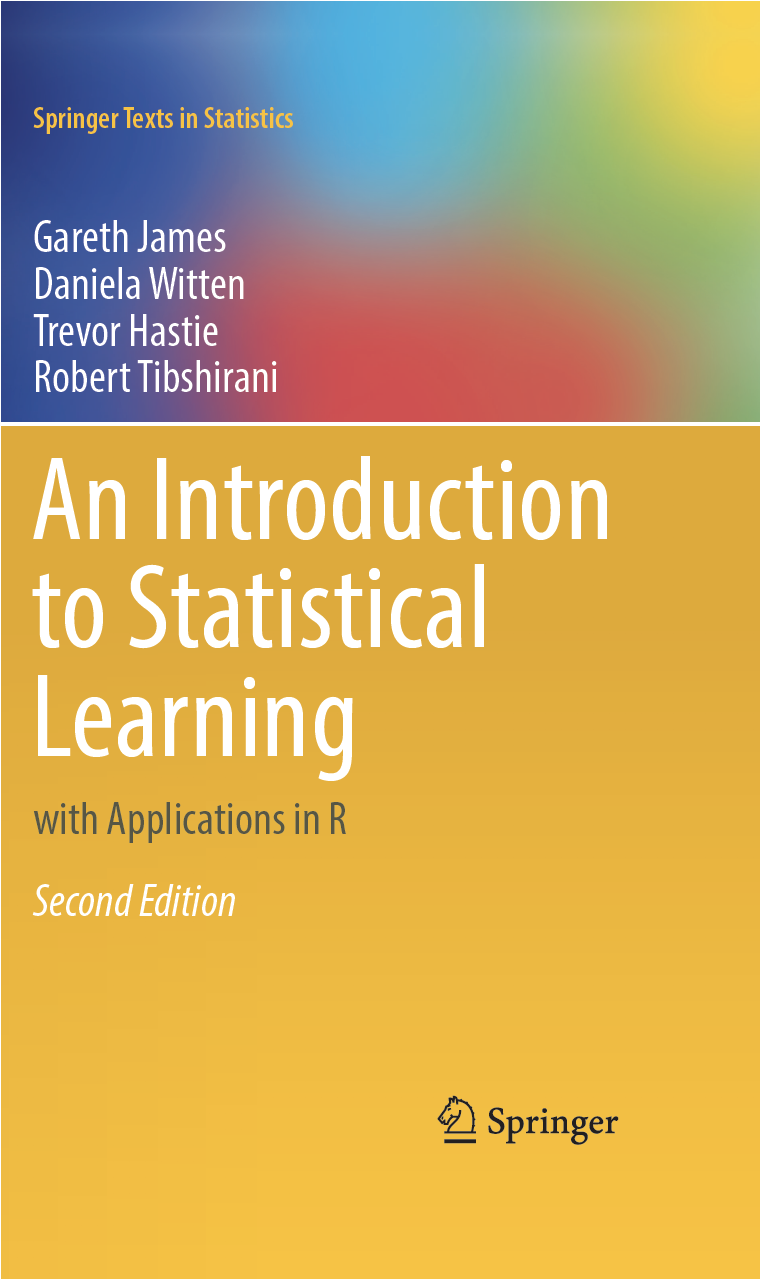
\includegraphics[height=0.7\textheight]{figures/book_cover} \\
    \vspace{4mm}
    {
        \tiny
        Content has been extracted from \textit{An Introduction to Statistical Learning with Applications in R}, Second Edition, by James, Witten, Hastie \& Tibshirani. Springer. 2023.\\
        Visit \url{https://www.statlearning.com/}.\\
    }
\end{frame}

\begin{frame}{Fitting Neural Networks}
    \begin{columns}[c]
        \begin{column}{0.48\textwidth}
            \centering
            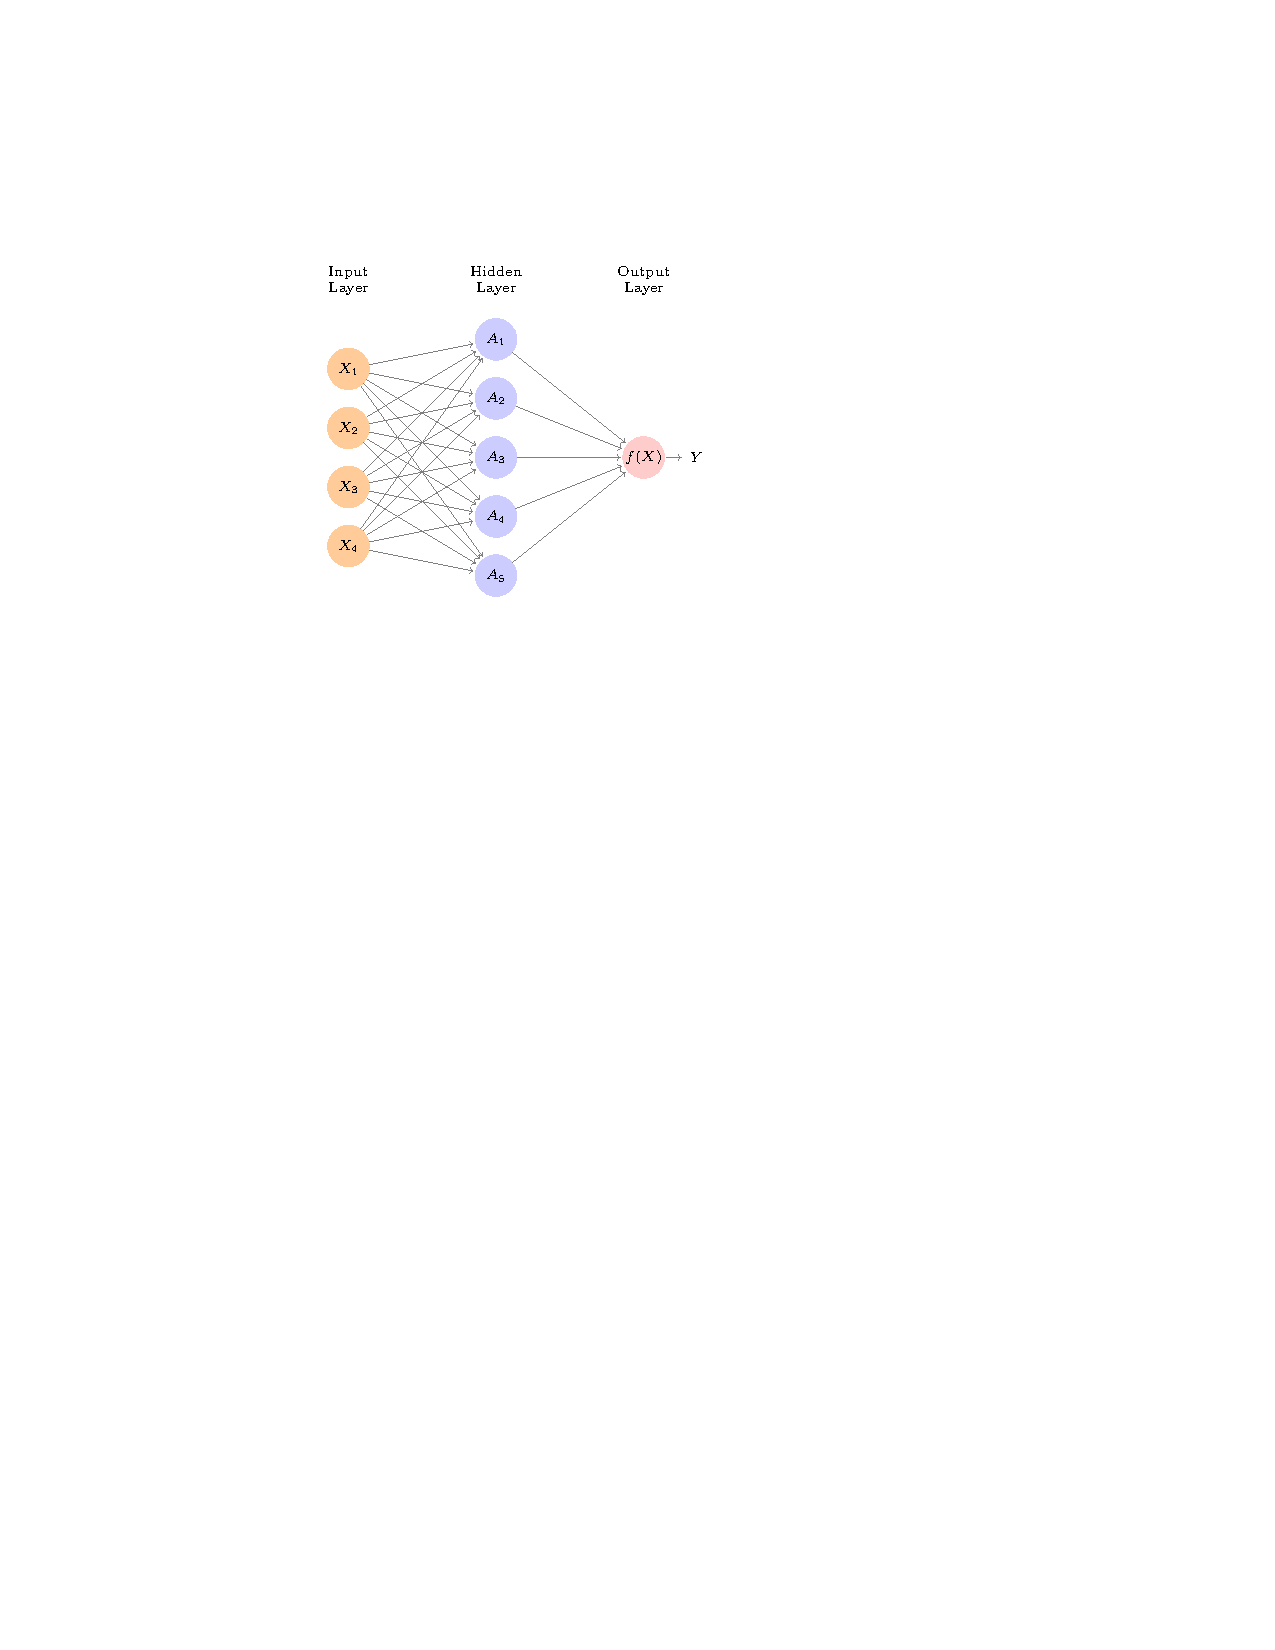
\includegraphics[trim={5cm 17cm 9cm 3cm}, clip, width=\textwidth]{figures/10_1.pdf}
        \end{column}
        \begin{column}{0.48\textwidth}
            \begin{equation*}
            \min_{\{w_{k}\}_{1}^{K},\beta}\frac{1}{2}\sum_{i=1}^{n}(y_{i}-f(x_{i}))^{2},
            \end{equation*}
            where
            \begin{equation*}
            f(x_{i})=\beta_{0}+\sum_{k=1}^{K}\beta_{k}g\left(w_{k0}+\sum_{j=1}^{p}w_{kj}x_{ij}\right).
            \end{equation*}
        \end{column}
    \end{columns}
    \footnotesize
    \pause
    This problem is difficult because the objective is \textbf{non-convex}. Despite this, effective algorithms have evolved that can optimize complex neural network problems efficiently.
\end{frame}

\begin{frame}{Non Convex Functions and Gradient Descent}
    Let $R(\theta)=\frac{1}{2}\sum_{i=1}^{n}(y_{i}-f_{\theta}(x_{i}))^{2}$ with $\theta=(\{w_{k}\}_{1}^{K},\beta).$

    \centering
    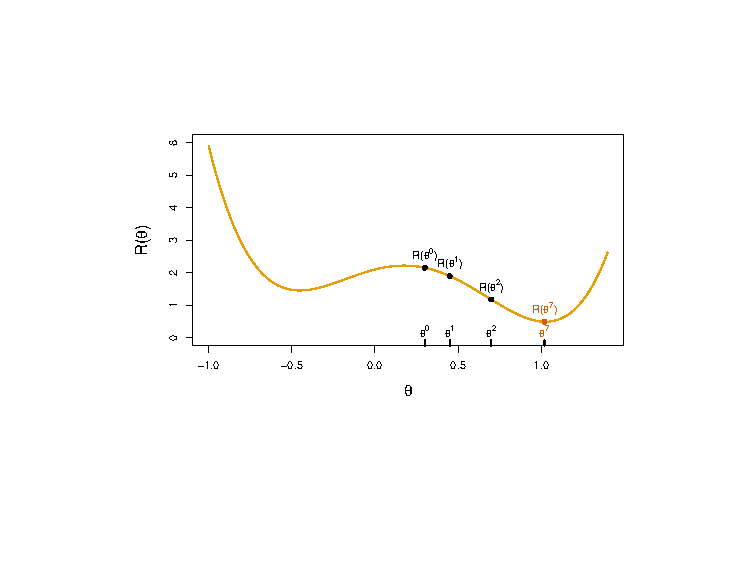
\includegraphics[width=0.65\textwidth]{figures/10_22.pdf}

    \begin{enumerate}
        \item Start with a guess $\theta^{0}$ for all the parameters in $\theta$, and set $t=0$.
        \item Iterate until the objective $R(\theta)$ fails to decrease:
        \begin{enumerate}
            \item Find a vector $\delta$ that reflects a small change in $\theta$, such that $\theta^{t+1}=\theta^{t}+\delta$ \textbf{reduces} the objective; i.e. $R(\theta^{t+1})<R(\theta^{t})$.
            \item Set $t \leftarrow t + 1.$
        \end{enumerate}
    \end{enumerate}
\end{frame}

\begin{frame}{Gradient Descent Continued}
    \small
    \begin{itemize}
        \item In this simple example we reached \textbf{the global minimum}.
        \item If we had started a little to the left of $\theta^{0}$ we would have gone in the other direction, and ended up in a \textbf{local minimum}.
        \item Although $\theta$ is multi-dimensional, we have depicted the process as one-dimensional. It is much harder to identify whether one is in a local minimum in high dimensions.
    \end{itemize}

    \vspace{1em}
    How to find a direction $\delta$ that points downhill? We compute the \textbf{gradient vector}
    \begin{equation*}
    \nabla R(\theta^{t})=\left.\frac{\partial R(\theta)}{\partial\theta}\right|_{\theta=\theta^{t}}
    \end{equation*}
    i.e. the vector of \textbf{partial derivatives} at the current guess $\theta^{t}.$

    \vspace{1em}
    The gradient points uphill, so our update is $\delta=-\rho\nabla R(\theta^{t})$ or
    \begin{equation*}
    \theta^{t+1}\leftarrow\theta^{t}-\rho\nabla R(\theta^{t})
    \end{equation*}
    where $\rho$ is the \textbf{learning rate} (typically small, e.g. $\rho=0.001$).
\end{frame}

\begin{frame}{Gradients and Backpropagation}
    $R(\theta)=\sum_{i=1}^{n}R_{i}(\theta)$ is a sum, so gradient is sum of gradients.

    \begin{equation*}
    R_{i}(\theta)=\frac{1}{2}(y_{i}-f_{\theta}(x_{i}))^{2}=\frac{1}{2}\left(y_{i}-\beta_{0}-\sum_{k=1}^{K}\beta_{k}g\left(w_{k0}+\sum_{j=1}^{p}w_{kj}x_{ij}\right)\right)^{2}
    \end{equation*}

    For ease of notation, let $z_{ik}=w_{k0}+\sum_{j=1}^{p}w_{kj}x_{ij}.$

    \vspace{1em}
    Backpropagation uses the \textbf{chain rule for differentiation}:
    \begin{align*}
    \frac{\partial R_{i}(\theta)}{\partial\beta_{k}}&=\frac{\partial R_{i}(\theta)}{\partial f_{\theta}(x_{i})}\cdot\frac{\partial f_{\theta}(x_{i})}{\partial\beta_{k}} \\
    &=-(y_{i}-f_{\theta}(x_{i}))\cdot g(z_{ik}).
    \end{align*}
    \begin{align*}
    \frac{\partial R_{i}(\theta)}{\partial w_{kj}}&=\frac{\partial R_{i}(\theta)}{\partial f_{\theta}(x_{i})}\cdot\frac{\partial f_{\theta}(x_{i})}{\partial g(z_{ik})}\cdot\frac{\partial g(z_{ik})}{\partial z_{ik}}\cdot\frac{\partial z_{ik}}{\partial w_{kj}} \\
    &=-(y_{i}-f_{\theta}(x_{i}))\cdot\beta_{k}\cdot g^{\prime}(z_{ik})\cdot x_{ij}.
    \end{align*}
\end{frame}

\begin{frame}{Tricks of the Trade}
    \begin{itemize}
        \item<1-> \textbf{Slow learning}. Gradient descent is slow, and a small learning rate $\rho$ slows it even further. With early stopping, this is a form of regularization.
        \item<2-> \textbf{Stochastic gradient descent}. Rather than compute the gradient using all the data, use a small minibatch drawn at random at each step. E.g. for MNIST data, with $n=60K$, we use minibatches of 128 observations.
        \item<3-> An \textbf{epoch} is a count of iterations and amounts to the number of minibatch updates such that $n$ samples in total have been processed; i.e. $60K/128\approx469$ for MNIST.
        \item<4-> \textbf{Regularization}. Ridge and lasso regularization can be used to shrink the weights at each layer. Two other popular forms of regularization are dropout and augmentation, discussed next.
    \end{itemize}
\end{frame}

\begin{frame}{Dropout Learning}
    \centering
    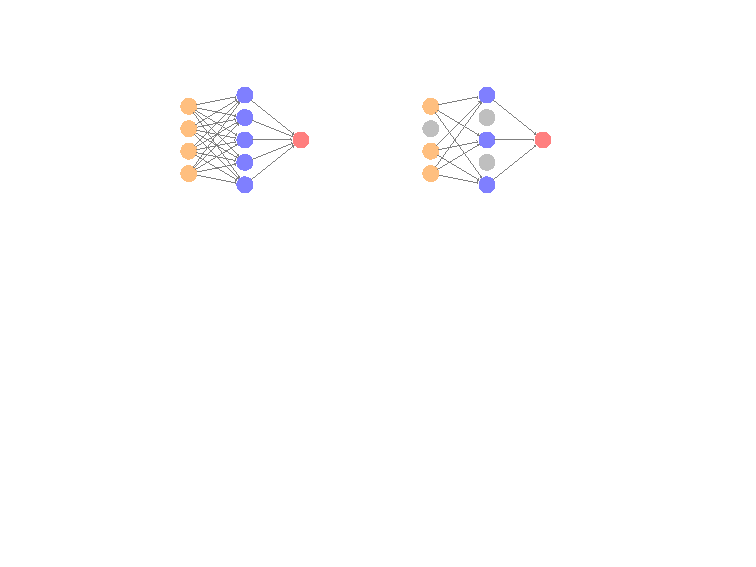
\includegraphics[width=0.75\textwidth]{figures/10_23}
    \begin{itemize}
        \item<1-> At each SGD update, randomly remove units with probability $\phi$, and scale up the weights of those retained by $1/(1-\phi)$ to compensate.
        \item<2-> In simple scenarios like linear regression, a version of this process can be shown to be equivalent to ridge regularization.
        \item<3-> As in ridge, the other units \textbf{stand in} for those temporarily removed, and their weights are drawn closer together.
        \item<4-> Similar to randomly omitting variables when growing trees in random forests (Chapter 8).
    \end{itemize}
\end{frame}

\begin{frame}{Ridge and Data Augmentation}
    \begin{columns}[c]
        \begin{column}{0.48\textwidth}
            \centering
            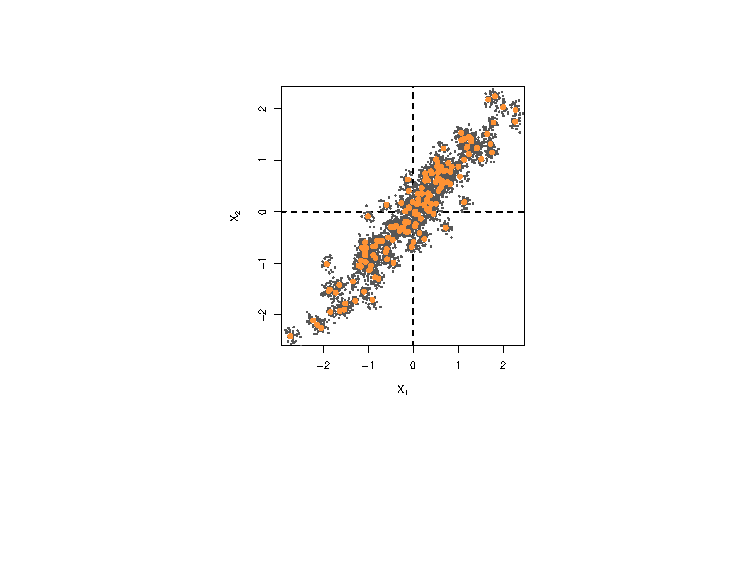
\includegraphics[width=\textwidth]{figures/10_24}
        \end{column}
        \begin{column}{0.48\textwidth}
            \begin{itemize}
                \item Make many copies of each $(x_{i},y_{i})$ and add a small amount of Gaussian noise to the $x_{i}$ -- a little cloud around each observation -- but leave the copies of $y$ alone!
                \item This makes the fit robust to small perturbations in $x_{i}$, and is equivalent to ridge regularization in an OLS setting.
            \end{itemize}
        \end{column}
    \end{columns}
\end{frame}

\begin{frame}{Data Augmentation on the Fly}
    \centering
    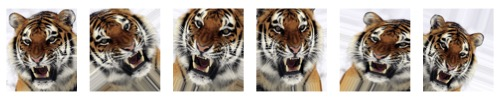
\includegraphics[width=\textwidth]{figures/10_9}
    \begin{itemize}
        \item<1-> Data augmentation is especially effective with SGD, here demonstrated for a CNN and image classification.
        \item<2-> Natural transformations are made of each training image when it is sampled by SGD, thus ultimately making a cloud of images around each original training image.
        \item<3-> The label is left unchanged in each case -- still tiger.
        \item<4-> Improves performance of CNN and is similar to ridge.
    \end{itemize}
\end{frame}

\begin{frame}{Software}
    \begin{itemize}
        \item Wonderful software available for neural networks and deep learning. \texttt{\textbf{Tensorflow}} from Google and \texttt{PyTorch} from Facebook. Both are \texttt{Python} packages.
        \item In the Chapter 10 lab we demonstrate \texttt{tensorflow} and \texttt{keras} packages in \texttt{R}, which interface to \texttt{Python}. See textbook and online resources for \texttt{Rmarkdown} and \texttt{Jupyter} notebooks for these and all labs for the second edition of ISLR book.
        \item The \texttt{torch} package in \texttt{R} is available as well, and implements the \texttt{PyTorch} dialect. The Chapter 10 lab will be available in this dialect as well; watch the resources page at \texttt{\url{www.statlearning.com}}.
    \end{itemize}
\end{frame}

\begin{frame}{}
    \centering
    \Huge End of Chapter 10.
\end{frame}

\begin{frame}{An Introduction to Statistical Learning with Applications in R}{a.k.a. ISLR}
    \centering
    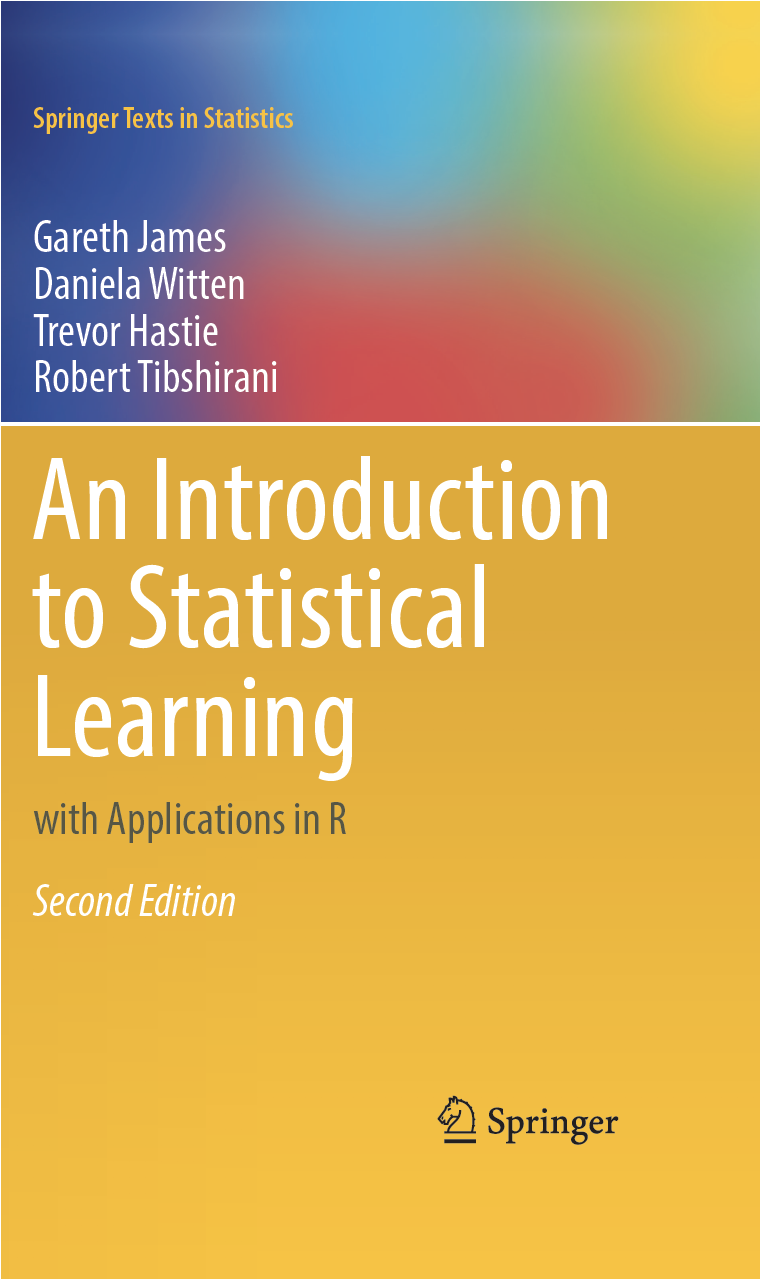
\includegraphics[height=0.7\textheight]{figures/book_cover} \\
    \vspace{4mm}
    {
        \tiny
        Content has been extracted from \textit{An Introduction to Statistical Learning with Applications in R}, Second Edition, by James, Witten, Hastie \& Tibshirani. Springer. 2023.\\
        Visit \url{https://www.statlearning.com/}.\\
    }
\end{frame}

\end{document}
